\documentclass[12pt]{article}
\usepackage[top=1in,left=1in, right = 1in, footskip=1in]{geometry}

\usepackage{graphicx}
\usepackage{xspace}
%\usepackage{adjustbox}

\newcommand{\comment}{\showcomment}
%% \newcommand{\comment}{\nocomment}

\newcommand{\showcomment}[3]{\textcolor{#1}{\textbf{[#2: }\textsl{#3}\textbf{]}}}
\newcommand{\nocomment}[3]{}

\newcommand{\jd}[1]{\comment{cyan}{JD}{#1}}
\newcommand{\swp}[1]{\comment{magenta}{SWP}{#1}}
\newcommand{\bmb}[1]{\comment{blue}{BMB}{#1}}
\newcommand{\djde}[1]{\comment{red}{DJDE}{#1}}

\newcommand{\eref}[1]{Eq.~\ref{eq:#1}}
\newcommand{\fref}[1]{Fig.~\ref{fig:#1}}
\newcommand{\Fref}[1]{Fig.~\ref{fig:#1}}
\newcommand{\sref}[1]{Sec.~\ref{#1}}
\newcommand{\frange}[2]{Fig.~\ref{fig:#1}--\ref{fig:#2}}
\newcommand{\tref}[1]{Table~\ref{tab:#1}}
\newcommand{\tlab}[1]{\label{tab:#1}}
\newcommand{\pday}{\ensuremath{/\textrm{day}}}

\usepackage{amsthm}
\usepackage{amsmath}
\usepackage{amssymb}
\usepackage{amsfonts}

\usepackage{lineno}
\linenumbers

\usepackage[pdfencoding=auto, psdextra]{hyperref}

\usepackage{natbib}
\bibliographystyle{chicago}
\date{\today}

\usepackage{xspace}
\newcommand*{\ie}{i.e.\@\xspace}

\usepackage{color}

\newcommand{\Rx}[1]{\ensuremath{{\mathcal R}_{#1}}\xspace} 
\newcommand{\Ro}{\Rx{0}}
\newcommand{\Rc}{\Rx{\mathrm{c}}}
\newcommand{\Ri}{\Rx{\mathrm{i}}}
\newcommand{\RR}{\ensuremath{{\mathcal R}}\xspace}
\newcommand{\Rhat}{\ensuremath{{\hat\RR}}}
\newcommand{\Rprop}{\Rx{\mathrm{prop}}}
\newcommand{\Rcori}{\Rx{\mathrm{cori}}}
\newcommand{\tsub}[2]{#1_{{\textrm{\tiny #2}}}}
\newcommand{\dd}[1]{\ensuremath{\, \mathrm{d}#1}}
\newcommand{\dtau}{\dd{\tau}}
\newcommand{\dx}{\dd{x}}
\newcommand{\dsigma}{\dd{\sigma}}

\newcommand{\tstart}{\ensuremath{\tsub{t}{start}}\xspace}
\newcommand{\tend}{\ensuremath{\tsub{t}{end}}\xspace}

\newcommand{\betaeff}{\ensuremath{\tsub{\beta}{eff}}\xspace}
\newcommand{\Keff}{\ensuremath{\tsub{K}{eff}}\xspace}
\newcommand{\Kpost}{\ensuremath{\tsub{K}{post}}\xspace}

\newcommand{\pt}{p} %% primary time
\newcommand{\st}{s} %% secondary time

\newcommand{\psize}{{\mathcal P}} %% primary cohort size
\newcommand{\ssize}{{\mathcal S}} %% secondary cohort size

\newcommand{\gtime}{\sigma} %% generation interval
\newcommand{\gdist}{g} %% generation-interval distribution

\newcommand{\geff}{g_{\textrm{eff}}} %% generation-interval distribution

\newcommand{\total}{{\mathcal T}} %% total number of serial intervals

\newcommand{\PP}{\ensuremath{\mathcal P}}
\newcommand{\II}{\ensuremath{\mathcal I}}
\newcommand{\HH}{\ensuremath{\mathcal H}}

\begin{document}

\begin{flushleft}{
	\Large
	\textbf\newline{
		Immune boosting bridges leaky and polarized vaccination models
	}
}
\newline
\\
Sang Woo Park\textsuperscript{1,*}, Chadi Saad-Roy, ???, Bryan T Grenfell, Jonathan Dushoff
\\
\bigskip
\textbf{1} Department of Ecology and Evolutionary Biology, Princeton University, Princeton, NJ, USA
\\
\bigskip

*Corresponding author: swp2@princeton.edu
\end{flushleft}

\section*{Introduction}

Vaccination plays a critical role in controlling infectious disease outbreaks by protecting against new infections \citep{iwasaki2020and}.
In particular, when a critical vaccination threshold is reached, the basic reproduction number (defined as the average number of secondary infections caused by an infected individual) is reduced to below 1, and future epidemics can be prevented \citep{anderson1985vaccination}.
But reaching a critical vaccination threshold is challenging, and vaccines often provide imperfect protections.

There are two main ways of modeling vaccines with imperfect protections: ``leaky'' and ``all-or-nothing'' vaccine \citep{smith1984assessment}.
The leaky vaccination model assumes that vaccinated individuals experience a reduced force of infection (for example, by a factor of $p < 1$).
On the other hand, the ``all-or-nothing'' vaccination model assumes that the proportion $p$ of vaccinated individuals are completely susceptible to infections and the remaining proportion $1-p$ of vaccinated individuals are completely protected.
This model is analogous to the polarized immunity model, in which infection from one strain gives complete or no protection against other strains \citep{gog2002dynamics}---following this convention, we refer to this model as the polarized vaccination model.

Even though two models seem to assume same values of vaccine efficacy, they predict different epidemic dynamics, including the final size \citep{smith1984assessment}:
all vaccinated individuals can eventually get infected in the leaky model, whereas some vaccinated individuals never get infected in the polarized model.
The polarized vaccination model can be also less realistic for many pathogens because vaccines often provide some sort of protection against infections for most individuals---we note that vaccines can fail and provide no protection at all in rare cases.
Therefore, modelers have often relied on the leaky assumptions, especially throughout the SARS-CoV-2 pandemic.
But the leaky model also relies implicitly on an unrealistic assumption---With probability $1-p$, individuals that are exposed to infections do not get infected and continue to remain as equally susceptible as before the exposure.
In practice, vaccinated individuals who successfully fight off exposures can experience immune boosting, through which they can become less susceptible (or even protected) to future infections without becoming infectious from the exposure.

In this study, we compare different models of vaccination.
First, we illustrate that the difference between the leaky vaccination model and the polarized vaccination models can be reconciled via immune boosting mechanism.
In doing so, we show that the polarized vaccination model and immune boosting model predict identical epidemic dynamics but different serological dynamics.
Then, we present a generalized vaccination model which bridges all three models and explore its dynamics.
Finally, we use our framework to compare two ways of measuring vaccine efficacy and show that leaky and polarized vaccination models each have a correct way of measuring vaccine efficacy.

\section*{Mathematical models of vaccine-induced immunity}

\begin{figure}[!th]
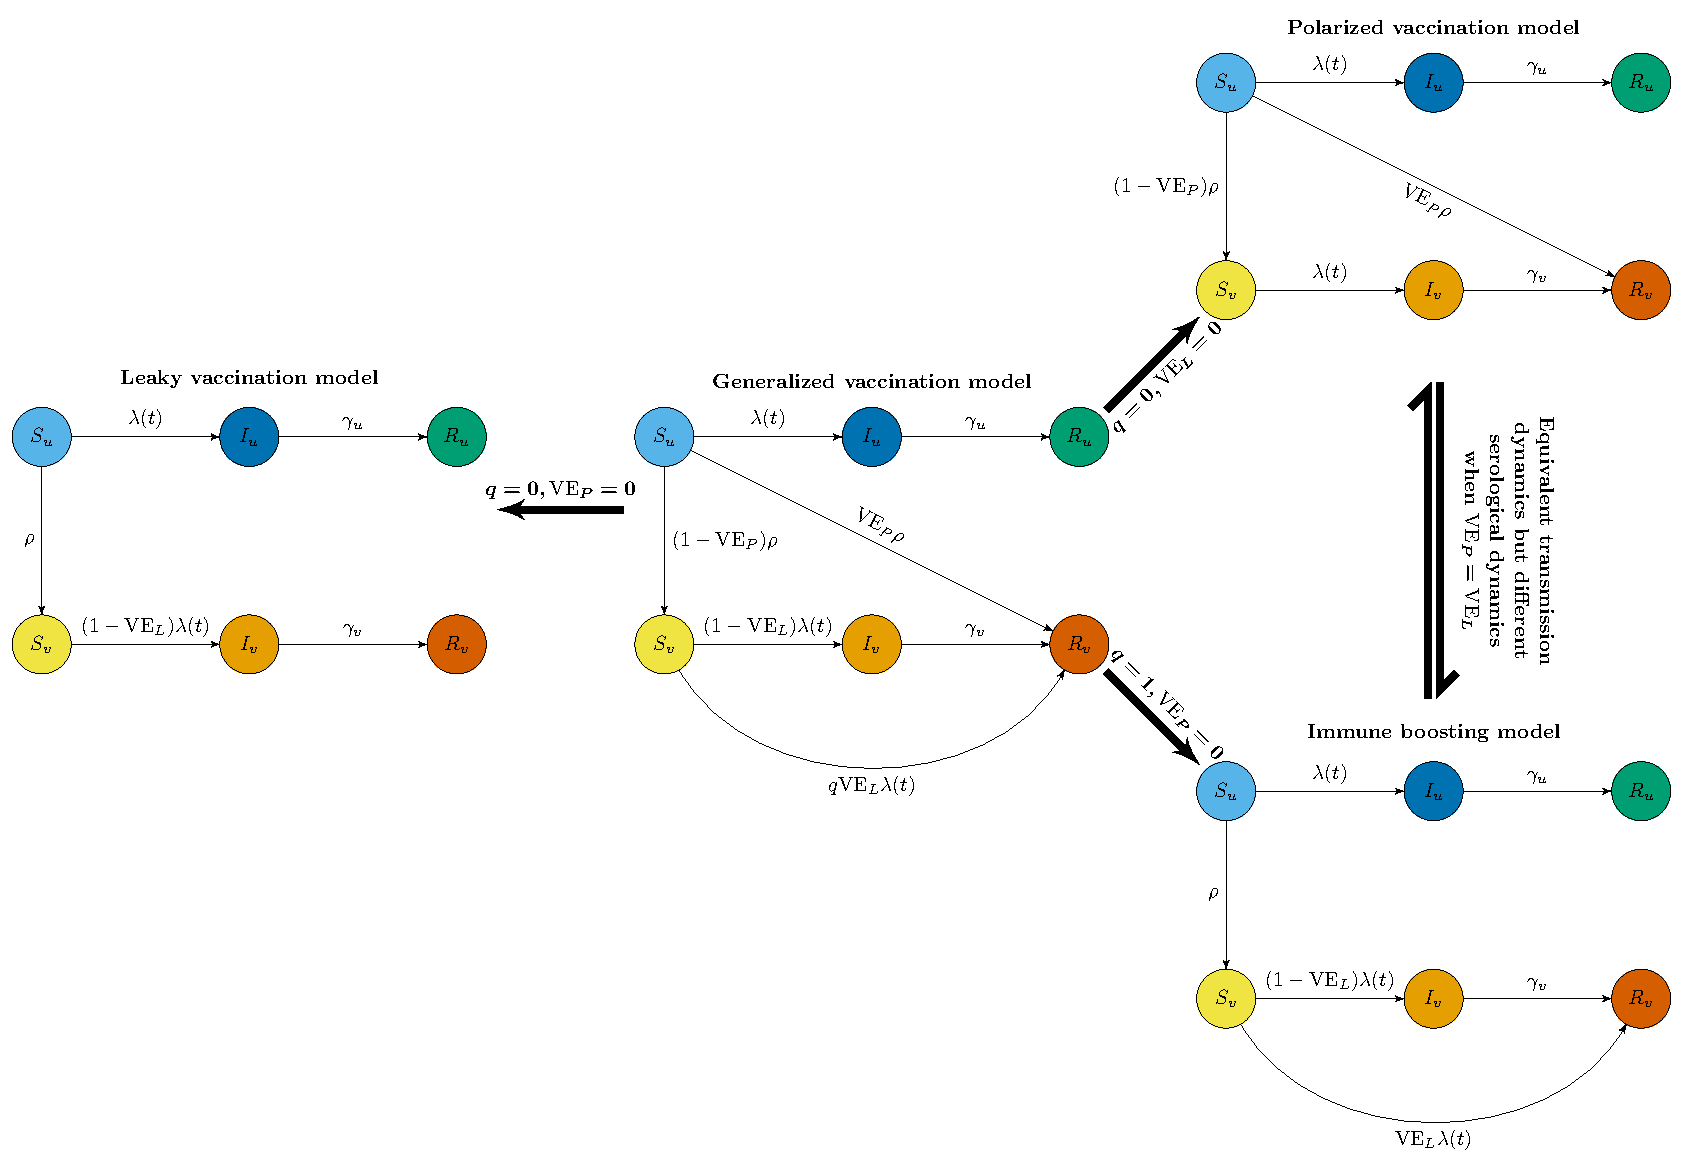
\includegraphics[width=\textwidth]{figure_diagram_comb.pdf}
\caption{
\textbf{A schematic diagram of vaccine models}
\label{fig:diagram}
}
\end{figure}

First, we begin with a standard SIR model with a leaky vaccine, in which all vaccinated individuals experience a reduced force of infection by a factor of $p$:
\begin{align}
\frac{\dd S_u}{\dd t} &= - \lambda(t) S_u - \rho S_u \\
\frac{\dd I_u}{\dd t} &= \lambda(t) S_u - \gamma_u I_u \\
\frac{\dd R_u}{\dd t} &= \gamma_u I_u \\
\frac{\dd S_v}{\dd t} &= - p \lambda(t) S_v + \rho S_u \\
\frac{\dd I_v}{\dd t} &= p \lambda(t) S_v - \gamma_v I_v \\
\frac{\dd R_v}{\dd t} &= \gamma_v I_v
\end{align}
where subscripts $u$ and $v$ indicate the unvaccinated and vaccinated individuals;
$\lambda$ represents the baseline force of infection experienced by unvaccinated individuals; 
$\rho$ represents vaccination rate;
and $\gamma$ represent the recovery rate.
This kind of model is also referred to as a history-based model as the susceptibility of an individual depends on the history of infections or vaccination---in this case, all individuals who have the same vaccine history have identical susceptibility \citep{gog2002dynamics,gog2002status,kucharski2016capturing}.
For this model, $1-p$ also represents the vaccine efficacy, which captures the amount of reduction in the probability of infection.

On the other hand, the polarized vaccination model assumes that a proportion $p$ of vaccinated individuals still remain susceptible, whereas the remaining proportion $1-p$ become fully immune: 
\begin{align}
\frac{\dd S_u}{\dd t} &= - \lambda(t) S_u - \rho S_u \\
\frac{\dd I_u}{\dd t} &= \lambda(t) S_u - \gamma_u I_u \\
\frac{\dd R_u}{\dd t} &= \gamma_u I_u \\
\frac{\dd S_v}{\dd t} &= - \lambda(t) S_v + p \rho S_u \\
\frac{\dd I_v}{\dd t} &= \lambda(t) S_v - \gamma_v I_v \\
\frac{\dd R_v}{\dd t} &= \gamma_v I_v + (1-p) \rho S_u
\end{align}
The polarized immunity model is often used in status-based models for cross immunity---the status-based models keep track of immune statuses of individuals, rather than their infection histories \citep{gog2002dynamics,gog2002status,kucharski2016capturing};
in this case, this model does not keep track of infection or vaccine history.
For this model, the parameter $1-p$ also provides some sort of measure for vaccine efficacy but has a different meaning from the parameter $p$ in the leaky vaccine model---we return to this point later.

While both the leaky vaccination model and the polarized vaccination model have been widely used in literature, their assumptions lead to a key dynamical differences: the leaky vaccination model assumes that all vaccinated individuals can be eventually infected, whereas the polarized vaccination model assumes that proportion $1-p$ of vaccinated individuals will never be infected.
In other words, the polarized vaccination model will always predict a lower final size than the leaky vaccination model.

To better understand these differences, we consider a immune boosting model.
The leaky vaccination model assumes that vaccinated individuals have an independent probability $p$ of infection for every challenge and will otherwise remain partially susceptible.
Instead, the immune boosting model assumes that unsuccessful challenges elicit immune response, moving individuals from $S_v$ to $R_v$ compartment at rate $(1-p) \lambda(t)$ and thereby breaking the independence assumption of the leaky vaccine model:  
\begin{align}
\frac{\dd S_u}{\dd t} &= - \lambda(t) S_u - \rho S_u \\
\frac{\dd I_u}{\dd t} &= \lambda(t) S_u - \gamma_u I_u \\
\frac{\dd R_u}{\dd t} &= \gamma_u I_u \\
\frac{\dd S_v}{\dd t} &= - \lambda(t) S_v + \rho S_u \\
\frac{\dd I_v}{\dd t} &= p \lambda(t) S_v - \gamma_v I_v \\
\frac{\dd R_v}{\dd t} &= (1-p) \lambda(t) S_v + \gamma_v I_v
\end{align}
In this model, both unvaccinated and vaccinated individuals are subject to identical forces of infections, which represent the per capita rate of challenges, but the outcome of challenges differ.
Since the depletion of vaccinated population $S_v$ always occurs at a faster rate under the immune boosting model than under the leaky vaccination model, the immune boosting model always predicts a lower final size.
Furthermore, epidemiological dynamics (i.e., trajectories of $I_u$ and $I_v$) predicted by the immune boosting model and the polarized vaccination model are identical: 
both models assume that individuals become vaccinated at rate $\rho$ and move out of the $S_v$ compartment at rate $\lambda$ and only differ in when individuals get sorted.
Such equivalence allows us to bridge the difference between the leaky and polarized vaccination models.
The equivalence holds regardless of infection characteristics of vaccinated individuals (i.e., the duration of their infection and their transmissibility);
however, it does not necessarily hold when immunity wanes as we discuss later.

Finally, we present a generalized vaccination model that encompasses all three models:
\begin{align}
\frac{\dd S_u}{\dd t} &= - \lambda(t) S_u - \rho S_u \\
\frac{\dd I_u}{\dd t} &= \lambda(t) S_u - \gamma_u I_u \\
\frac{\dd R_u}{\dd t} &= \gamma_u I_u \\
\frac{\dd S_v}{\dd t} &= - [q \{1-(p/\theta)\} + (p/\theta)] \lambda(t) S_v + \theta \rho S_u \\
\frac{\dd I_v}{\dd t} &= (p/\theta) \lambda(t) S_v - \gamma_v I_v \\
\frac{\dd R_v}{\dd t} &= (1 - \theta) \rho S_u + q [1-(p/\theta)] \lambda(t) S_v + \gamma_v I_v
\end{align}
This model includes two additional parameters: $\theta$ and $q$.
The parameter $\theta$ represents the proportion of individuals that remain partially susceptible after vaccination;
this parameter also scales the force of infection, allowing us to bridge the polarized vaccination and immune boosting models.
For example, when $\theta = 1$, all vaccinated individuals are partially susceptible to breakthrough infections;
the value of parameter $q$, which represents the proportion of unsuccessful challenges that result in immune boosting, allows us to bridge between the leaky vaccination model ($q=0$) and the immune boosting model ($q = 1$).
When $\theta = p$, a proportion $p$ of vaccinated individuals are completely susceptible to breakthrough infections, yielding a polarized vaccination model.
We note that this generalized model does not account for the possibility that a proportion $p$ of vaccinated individuals remain partially susceptible to breakthrough infections while the remaining proportion $1-p$ of vaccinated individuals are completely protected; 
as we will discuss later, a such model violates the definition of vaccine efficacy against infection.
These four models are summarized in \fref{diagram}.

\section*{Model simulations}

As an example, we assume that both unvaccinated and vaccinated individuals transmit at the same rate for an average of 5 days with $\mathcal R_0 = 2.5$ in a homogeneously mixing population.
For simplicity, we assume that 50\% individuals are vaccinated at the beginning of an epidemic with 60\% efficacy ($p=0.4$) and do not model vaccination during an outbreak ($\rho = 0$).
For the leaky vaccination model and the immune boosting model, we set $S_v(0) = 0.5$ as our initial condition.
For the polarized vaccination model, we set $S_v(0) = 0.5 p$ and $R_v(0) = 0.5 (1-p)$ as our initial condition.

\fref{simulation} compares epidemiological (A--C) and serological (D--F) trajectories predicted by three models (leaky vaccination model, polarized vaccination model, and immune boosting model).
As explained earlier, the leaky vaccination model predicts a larger outbreak with a slower decay rate among vaccinated individuals than predicted by both the polarized vaccination and immune boosting models;
the latter two models predict identical epidemic trajectories.
In this case, the leaky vaccination model also predicts a larger outbreak among unvaccinated individuals because a larger outbreak among vaccinated individuals causes unvaccinated individuals to also experience a greater forces of infection over time.

We also find that all three models predict different serological trajectories. (\fref{simulation}D--F).
The leaky vaccination model predicts the largest outbreak and therefore the highest levels of seroprevalence (89.7\% by the end of the simulation).
The immune boosting model predicts a slightly lower seroprevalence overall (85.6\%);
in addition, a higher proportion of vaccinated individuals have moved from $S_v$ to $R_v$ compartment through boosting.
The polarized vaccination model predicts an even lower seroprevalence (79.9\%) because individuals in the $S_v$ have not retained any immunity from the vaccination.

\begin{figure}[!th]
\includegraphics[width=\textwidth]{figure_simulation_compare.pdf}
\caption{
\textbf{Simulations of three different vaccination models}
\label{fig:simulation}
}
\end{figure}

We then use the generalized vaccination model to further investigate how the final size of the an epidemic among vaccinated individuals depends on assumptions about vaccine-derived immunity across a wide range of assumptions about the basic reproduction number $\mathcal R_0$ and vaccine efficacy $p$ (\fref{sensitivity}).
First, when all vaccinated individuals have identical susceptibility ($\theta = 1$), increasing the amount of boosting reduces the final size as expected (see first column of \fref{sensitivity}).
We observe biggest effects of boosting at intermediate vaccine efficacy, $p$, and high basic reproduction number, $\mathcal R_0$.
When vaccine efficacy is too low (or too high), then boosting has negligible effects because everyone (or no one) gets infected.
As we increase $\mathcal R_0$, the leaky vaccination model predicts that all vaccinated individuals will eventually get infected.
On the other hand, the final size predicted by the immune boosting model cannot be greater than $1-p$.
As we decrease $\theta$ from 1 to $p$, the generalized vaccination model collapses to the polarized vaccination model, and the final size becomes insensitive to the insensitive to the boosting parameter $q$.

\begin{figure}[!th]
\includegraphics[width=\textwidth]{figure_simulation_generalized_vaccinated.pdf}
\caption{
\textbf{Sensitivity of the final size of an outbreak among vaccinated individuals to assumptions about vaccine-derived immunity}
\label{fig:sensitivity}
}
\end{figure}

Finally, different assumptions about vaccination have important implications for measuring vaccine efficacy.
All of the models we presented so far seem to assume same values for the vaccine efficacy ($1-p$) but predict different dynamics. 
So how do we accurately estimate, or even define, vaccine efficacy?

Here, we compare two ways of estimating vaccine efficacy: the ratios of cumulative incidence and instantaneous hazard.
The cumulative incidence refers to the cumulative proportion of infections among unvaccinated and vaccinated individuals; 
this is typically used for measuring the vaccine effectiveness from real-life outbreaks.
To calculate the cumulative-incidence-based estimates of vaccine efficacy from our general model, we add two additional compartments, which keep track of cumulative incidence among unvaccinated $C_u$ and vaccinated $C_v$ individuals:
\begin{align}
\frac{\dd C_u}{\dd t} &= \lambda S_u\\
\frac{\dd C_v}{\dd t} &= (p/\theta) \lambda S_v
\end{align}
Then, the cumulative proportion of infections among vaccinated $p_v(t)$ and unvaccinated $p_u(t)$ individuals can be expressed as:
\begin{align}
p_u(t) &= C_u(t)/S_u(0)\\
p_v(t) &= C_v(t)/S_v(0)
\end{align}
Then, the estimated vaccine efficacy at time $t$ corresponds to:
\begin{equation}
1 - \frac{p_v(t)}{p_u(t)}.
\end{equation}

On the other hand, instantaneous hazard refers to the per-capita rate at which unvaccinated $h_u(t)$ and vaccinated $h_v(t)$ individuals get infected if they have not yet been infected yet.
Calculating the per-capita rate of infection among vaccinated individuals is tricky because boosted individuals have not been infected yet, even though they have been exposed; therefore, boosted individuals would still be included in the denominator when we calculate the per-capita rate of infection $i_v(t)$ among vaccinated individuals:
\begin{equation}
i_v(t) = \frac{(p/\theta) \lambda(t) S_v(t)}{S_v(0) - C_v(t)},
\end{equation}
where $S_v(0) - C_v(t) \geq S_v(t)$ because vaccinated individuals can leave the $S_v(t)$ compartment via boosting.
The per-capita rate of infection $i_u(t)$ among unvaccinated individuals is straightforward: 
\begin{equation}
i_u(t) = \frac{\lambda(t) S_u(t)}{S_u(t)} = \lambda(t).
\end{equation}
Then, the estimated vaccine efficacy at time $t$ corresponds to:
\begin{equation}
1 - \frac{i_v(t)}{i_u(t)}.
\end{equation}

We compare two estimates of vaccine efficacy across a wide range of assumptions about vaccine-derived immunity in \fref{efficacy}.
We assume 60\% efficacy throughout (therefore $p = 0.4$).
When all unsuccessful challenges result in immune boosting ($q=1$, immune boosting model in \fref{diagram}), the cumulative-incidence-based estimates always give correct answers throughout the epidemic---since the susceptible pool among unvaccinated and vaccinated individuals is depleted at the same rate $\lambda$, the ratios of their proportions of cumulative infections remain constant.
Likewise, the cumulative incidence-based estimates also give correct answers for the polarized vaccination model ($\theta = p$).
However, when some challenges are not boosted ($q < 1$), using cumulative incidence underestimates the vaccine efficacy beyond the exponential growth phase.
This is because vaccinated individuals who have been exposed but are not boosted or infected still remain susceptible to future infections; 
larger final epidemic sizes predicted by these models (\fref{sensitivity}) then translate to a seemingly lower vaccine efficacy.

The hazard-based estimates give correct answers for the leaky vaccine model (when $q=0$ and $\theta=1$) because the ratios of force of infection that unvaccinated and vaccinated individuals experience are always constant.
However, the using hazard ratios overestimates vaccine efficacy in the presence of immune boosting: since boosted individuals have not yet been infected, the susceptible pool in the vaccinated group appears to be bigger than it really is, causing the per-capita rate of infection to seem smaller.
Vaccine efficacy is also overestimated for polarized vaccination for similar reasons.

We note that both estimates give correct answers regardless of underlying assumptions about immunity during the exponential growth phase.
More generally, we expect both estimates to give unbiased estimates as long as the depletion of susceptible pool is negligible among both vaccinated and unvaccinated individuals;
in trial settings, where incidence is relatively low, this assumption may hold.
But estimating vaccine efficacy from real outbreaks is expected to be more difficult especially when the disease is spreading rapidly and causing susceptible depletion.

Finally, we note, again, that the generalized model does not account for the possibility that the proportion $p$ of vaccinated individuals remain partially susceptible to breakthrough infections while the remaining proportion $1-p$ of vaccinated individuals are completely protected (through polarization).
The standard polarized vaccination model, in which the proportion $p$ of vaccinated individuals are completely susceptible and the remaining proportion $1-p$ are fully protected, assume vaccine efficacy of $1-p$, which can be correctly estimated using both estimators during the exponential growth phase (\fref{efficacy}).
However, if the proportion $p$ of vaccinated individuals were less susceptible (as in the leaky sense), a such model would have an even higher vaccine efficacy, thereby violating our assumptions.

\begin{figure}[!th]
\includegraphics[width=\textwidth]{figure_simulation_efficacy.pdf}
\caption{
\textbf{Sensitivity of the final size of an outbreak among vaccinated individuals to assumptions about vaccine-derived immunity}
\label{fig:efficacy}
}
\end{figure}

\section*{Discussion}

Understanding the degree to which vaccination provides protection against infections is critical to predicting their population-level impact on epidemic dynamics.
Two models of vaccine-derived immunity have been previously proposed: leaky and polarized vaccination models.
The polarized model has been largely neglected in epidemiological modeling due to its extreme assumptions that a fraction of vaccinated individuals do not attain any protection. 
But the leaky vaccination model also makes an unrealistic assumption that vaccinated individuals who are exposed to infections can still remain susceptible, independent of previous exposures; 
a such assumption causes the leaky vaccination model to always predict a larger epidemic final size.
The differences in their epidemic dynamics can be understood by immune boosting: vaccinated individuals can attain protection without developing a transmissible infection, and therefore their infections are no longer independent of their previous exposures.
In particular, the immune boosting model predicts identical epidemic dynamics as the polarized vaccination model because the number of individuals who develop complete protection from polarization is equal to to the number of individuals who are boosted through exposure.


We also present a generalized vaccination model, which captures the dynamics of all three models.
Even though immune boosting and polarized vaccination models predict the same epidemic dynamics, they have different serological dynamics---these differences can be bridged by the generalized vaccination model.
The generalized vaccination model includes two additional parameters, which determine the amount of immune boosting and the proportion of individuals that remain partially susceptible after vaccination (rather than fully protected).
Using the generalized vaccination model, we show that the epidemic dynamics are most sensitive to the assumptions about vaccine-derived immunity at a intermediate vaccine efficacy.

Previous studies have tried to understand the differences between leaky and polarized vaccination models using arguments based on heterogeneity in susceptibility.
For example, leaky vaccination represents one extreme in which everyone has identical susceptibility;
polarized vaccination represents another exmtreme in whiche vaccinated individuals are either completely susceptible or not susceptible.
\cite{gomes2014missing} tried to reconcile these two assumptions by using a smooth distribution of susceptibility that changes from a delta distribution (leaky vaccination) to a polarized distribution;
however, they found that the predicted epidemic dynamics do not converge even though the distributions converge.
Our framework provides a simple explanations for these discrepancies:
regardless of the shape of the distribution of susceptibility, the leaky vaccination model always assumes that the infection events are independent of previous exposures.
On the other hand, the polarized distribution scenario no longer assumes independence because all exposures result in successful infections (for susceptible, vaccinated individuals).
In fact, the shape of the susceptibility distribution does not matter under immune boosting.
In Supplementary Materials, we provide a mathematical proof that the epidemic dynamics only depend on the mean susceptibility and are independent of the shape of the  susceptibility distribution immune boosting is included in the leaky vaccination model; we also present simulations to further illustrate the equivalence.
Therefore, we argue that neglecting immune boosting can lead to misleading conclusions about the effects of susceptibility heterogeneity in epidemic dynamics.\swp{maybe too strong?}

Finally, assumptions about vaccine-derived immunity also have important implications for estimating vaccine efficacy.
Vaccine efficacy can be estimated based on either the cumulative incidence or hazard rates.
The cumulative-incidence-based estimates give correct answers for polarized vaccination and immune boosting models,
whereas the hazard-based estimates give correct answers for the leaky vaccination model.
Neither methods give correct answers for intermediate cases in which there is partial polarization or boosting.
Nonetheless, both methods give correct estimates of vaccine efficacy for all vaccination models when susceptible depletion is negligible.
Therefore, vaccine efficacy and effectiveness estimates should be interpreted with care, especially when a large fraction of vaccinated individuals have been infected.

We rely on a simplifying assumption that natural infections (as well as polarized vaccination and immune boosting) provide complete protection against future infections.
In practice, both infection- and vaccine-derived immunity wanes over time for many pathogens.
When immunity wanes, polarized vaccination and immune boosting models may not necessarily predict identical dynamics.
In particular, individuals who gain complete protection through polarized immunity immediately enter the $R_v$ compartment upon vaccination, whereas those who gain complete protection through immune boosting take longer to enter the $R_v$ compartment because they need to be exposed to infections.
These differences can translate to shorter delays between reinfection events for the polarized immunity model, which in turn can lead to dynamical differences at the population level.
There are also other complexities that need to be considered.
For example, individuals who are boosted after vaccination can have different immunity profiles compared to those who attained strong protection from vaccination alone.
These individuals also likely have different immunity profiles from those who have been infected but never been vaccinated.
These differences can also cause polarized vaccination and immune boosting models to behave differently.
Despite these limitations, immune boosting, which is often neglected in epidemic models of vaccination, is still expected to be an important mechanism for understanding dynamics of many pathogens.

We have provided a unifying framework for understanding the impact of vaccination on the spread of infectious disease.
\swp{concluding paragraph please...}

\pagebreak

\section*{Supplementary Text}


Consider a immune boosting model that allows for heterogeneity in vaccine-derived immunity.
We assume that a vaccinated individual's susceptibility $0 \leq p \leq 1$ follows some distribution $f(p)$:
\begin{align}
\frac{\dd S_u}{\dd t} &= - \lambda(t) S_u - \rho S_u \\
\frac{\dd I_u}{\dd t} &= \lambda(t) S_u - \gamma_u I_u \\
\frac{\dd R_u}{\dd t} &= \gamma_u I_u \\
\frac{\partial S_v(p)}{\partial t} &= - \lambda(t) S_v(p) + f(p) \rho S_u  \\
\frac{\partial I_v(p)}{\partial t} &= p \lambda(t) S_v(p) - \gamma_v I_v(p) \\
\frac{\dd R_v}{\dd t} &= \int_0^1 \left[ (1-p) \lambda(t) S_v(p) + \gamma_v I_v(p) \right]\dd p
\end{align}
Due immune boosting, $S_v(p)$ is always depleted at a per-capita rate of $\lambda(t)$ regardless of the values of $p$, meaning that the (normalized) distribution of $S_v(p)$ will always follow $f(p)$.
To obtain the dynamics of total prevalence $I_v = \int I_v(p) \dd p$, we can integrate $\partial I_v(p)/\partial t$ across $p$:
\begin{align}
\frac{\dd I_v}{\dd t} &=  \int_0^1\left[\frac{\partial I_v(p)}{\partial t}\right]\dd p\\
&= \int_0^1\left[p \lambda(t) S_v(p) - \gamma_v I_v(p)\right]\dd p\\
&= \int_0^1\left[p f(p) \lambda(t) S_v - \gamma_v I_v(p)\right]\dd p\\
&= \bar{p} \lambda(t) S_v - \gamma_v I_v,
\end{align}
where $\bar{p}$ represents the mean of the distribution $f(p)$, and $S_v = \int S_v(p) \dd p$ represents the proportion of total susceptible, vaccinated individuals.
Therefore, the dynamics of total prevalence $I_v$ depends only on the mean susceptibility $\bar{p}$ and not on the shape of the distribution $f(p)$ under immune boosting.

\pagebreak

\bibliography{immune_boosting}

\end{document}
